\documentclass{article}
\usepackage{graphicx} % Required for inserting images

\title{Use Of Jigsaw Puzzle Solving Algorithms In The Real World}
\author{Luca Sartore}
\date{May 2023}

\begin{document}

\maketitle

\newpage

\tableofcontents

\newpage

\section{Abstract}
The jigsaw puzzle problem has been in the eye of computer scientists for a while,
and some clever solutions have already been found. These algorithms are made to
work with a “digital” jigsaw puzzle [Figure \ref{fig:figure_digital_puzzle}], there aren't papers
(at least not popular enough to be searchable) that try to apply the solution
to a “real world” (insert reference here) jigsaw puzzle.\newline
The problem has been tackled by some small projects. But, as said earlier,
the process and eventual challenges has never been documented by a paper,
this wants to be the first.\newline
As a Bonus the paper will also cover the creation of a user friendly app
that will be open source and free to use.

\section{Introduction}
\subsection{Classification}
This paper will focus on type 2 puzzles. A type 2 puzzle is a puzzle where the position, and the orientation of each piece is unknown. 
\subsection{Digital vs Real-World Jigsaw Puzzles}

There is  another important distinction between different types of puzzles. They can be divided into “digital” and “real world” jigsaw puzzles.

\bigskip

%\begin{center}

    
    \begin{figure}[h]
        \caption{An example of a “digital” puzzle}
        \label{fig:figure_digital_puzzle}
        \centering
        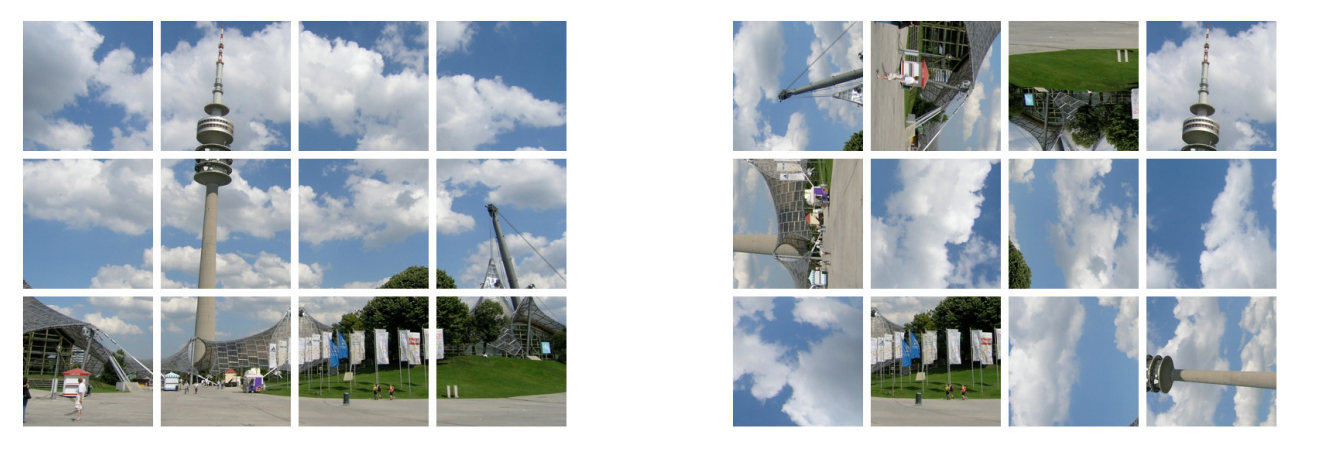
\includegraphics[width=0.5\textwidth]{pictures/digital_puzzle.png}
    \end{figure}

    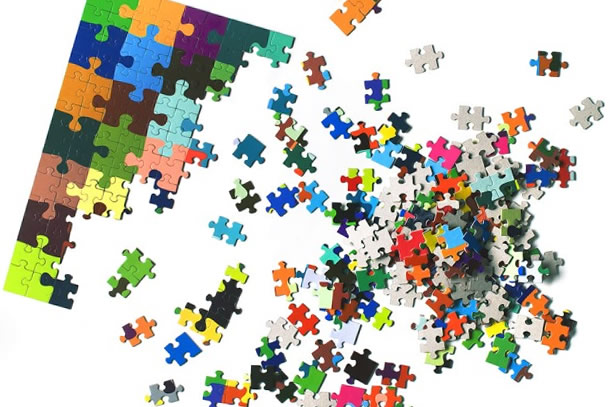
\includegraphics[height=0.3\columnwidth]{pictures/real_puzzle.jpg}
    \newline
    %\bigskip
    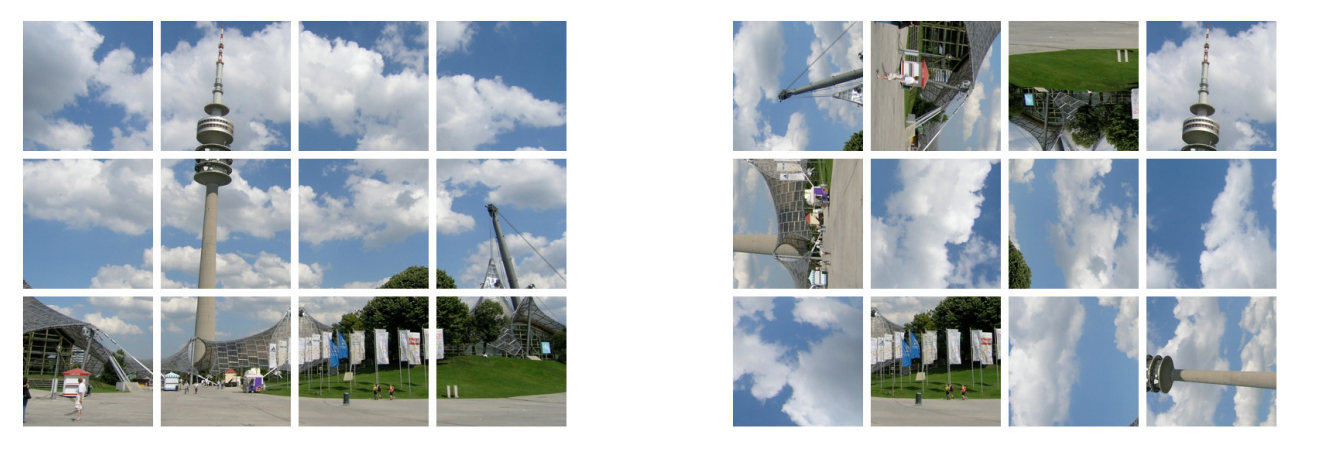
\includegraphics[height=0.3\columnwidth]{pictures/digital_puzzle.png}
%\end{center}


\end{document}
